\documentclass[conference,a4paper]{IEEEtran}
\IEEEoverridecommandlockouts

\usepackage[T1]{fontenc}
\usepackage[utf8]{inputenc}
\usepackage{cite}
\usepackage{amsmath,amssymb,amsfonts}
\usepackage{algorithmic}
\usepackage{graphicx}
\usepackage{textcomp}
\usepackage{xcolor}
\usepackage{booktabs}
\usepackage{array}
\usepackage{tabularx}
\usepackage{url}
\usepackage{listings}
\usepackage{tikz}

\lstdefinestyle{codestyle}{
  basicstyle=\ttfamily\footnotesize,
  breaklines=true,
  frame=single,
  columns=fullflexible,
  keepspaces=true,
  showstringspaces=false
}
\lstset{style=codestyle}

\begin{document}

\title{Mobility Diary: A Context-Aware System for Mobile Trip Acquisition, Activity Recognition, and Privacy-Aware Mobility Analysis}  \author{ \IEEEauthorblockN{Giacomo Bianco} \IEEEauthorblockA{\textit{Department of Computer Science and Engineering}\\ \textit{University of Bologna}\\ Bologna, Italy} }  \maketitle  \begin{abstract} This paper presents Mobility Diary, a context-aware mobility system designed to acquire, synchronize and visualize personal movement episodes collected through a mobile device. The system addresses the problem of battery-constrained and intermittently available mobile sensor data into a structured mobility diary that can be inspected by the user and, when needed, shared through privacy-aware representations. The proposed architecture combines on-device acquisition, finite-state tracking control, asynchronous backend ingestion, geospatial storage, Human Activity Recognition, significant-place mining, and multi-level privacy transformations.  The mobile app uses a finite-state machine to determine whether the user is stationary or in motion and collects GPS and sensor data. The backend receives trip data through a data ingestion workflow, inserts the visible trips into a PostgreSQL/PostGIS database, and processes the raw sensor data asynchronously using Celery workers. Human activity recognition is performed using a CNN-based feature extractor and a GRU temporal model, which produces semantic mobility segments such as walking, running, cycling, vehicle movement, and periods of inactivity. Recurring visits are then extracted from the raw GPS data to infer the user’s habitual locations. Finally, the activity log itself can be exported at different privacy levels, ranging from a detailed personal view to an approximate or aggregated view. \end{abstract}  \begin{IEEEkeywords} context-aware systems, mobile sensing, mobility diary, Human Activity Recognition, geolocation, PostGIS, asynchronous ingestion, privacy-aware data sharing, significant-place detection , Flutter, Django, Vue.js \end{IEEEkeywords}  \section{Introduction}  Modern smartphones continuously generate contextual signals that can be used to infer how people move through urban environments. GPS locations and inertial measurements provide sufficient information to detect stops, estimate modes of transportation, and identify frequently visited locations. However, transforming these raw signals into a reliable user diary is no trivial task. Mobile tracking is affected by battery limitations, sensor noise, operating system interruptions, variations in data arrival and privacy risks. A context-aware mobility system must therefore address both an inference problem and a systems engineering problem.  The Mobility Diary project was developed to address this challenge. The goal is to create an end-to-end system in which a mobile app records mobility events, a backend platform stores and processes them, and user-facing interfaces present the resulting diary through maps, timelines, statistics, significant locations, and privacy-compliant exports. The system goes beyond simple GPS tracking; instead, it aims to produce a semantic diary in which each trip is represented as a sequence of intervals, specifying stops, durations, recognized activities, and information about recurring locations.  A fundamental design requirement is that data acquisition must remain feasible on an actual mobile device. Continuous, high-frequency monitoring would provide highly detailed data, but it would also result in excessive battery drain and generate too much unnecessary data when the user is stationary. For this reason, the mobile app uses a finite-state acquisition model. The device distinguishes between stationary and moving states. In stationary conditions the app applies a low-power sampling profile and does not store sensor windows; when motion is confirmed it switches to a higher-frequency profile and begins persisting GPS points and inertial data. This approach reflects a fundamental principle of context-aware systems: sensing should be adapted to the context rather than performed uniformly at all times.  Another key requirement is reliability: a trip must not be lost if the network is temporarily unavailable, if the app is interrupted, or if the backend needs time to process large amounts of data. Evidence is therefore stored on the device first and uploaded only after the trip is closed, following a local-first, retryable synchronization strategy. Synchronization is split into two phases. A core phase transfers the minimum data required to make a trip visible in the diary, primarily GPS points and state transitions; a raw phase transfers the much larger inertial-sensor datasets. This separation lets the user see the recorded trip as soon as the core data is synchronized, while the raw sensor data is processed asynchronously on the backend to build the enriched diary. Moving the heavy work off the request path in this way also gives the system retries, idempotency, and workload isolation, instead of blocking mobile interactions on expensive machine-learning inference.  Human Activity Recognition is used as a semantic refinement layer rather than as the primary authority for trip lifecycle decisions. The mobile finite-state machine has priority at the operational level: it determines whether the device is in a stationary condition or whether a mobility episode should be tracked, using fixed  rules based on GPS speed and acceleration variance. Once a trip has been identified, the HAR pipeline operates at a finer temporal granularity. Its role is not to decide whether the trip exists, but to describe what happened inside the time interval accepted by the FSM as mobility evidence. Therefore, even within a tracked trip, HAR may identify short idle intervals, temporary stops, walking segments, cycling segments, running segments, or vehicle movement. This hierarchy prevents isolated HAR misclassifications from opening or closing trips, while still allowing the final diary to represent detailed sub-intervals that the rule-based FSM does not find.  Finally, the system includes a user-configurable privacy setting. Upon first login, the user chooses from three levels: precise, approximate, and aggregated. The precise level retains the complete personal log with actual trajectories and exact location information. The approximate level still tells the story of the trip in chronological order, but it makes the spatial information less identifiable: the path is moved to coarse spatial cells and meaningful places are replaced by generic labels such as residential area, university area, work area, or visited area. The aggregated level no longer describes the trip as a sequence of events, instead it publishes only summaries, such as time spent moving or stopped, prevalent activity and approximate distance ranges. In this design, privacy is applied as a final projection over the already enriched diary. The system therefore avoids rerunning asynchronous ingestion, HAR classification, segment construction, and significant-place mining for each privacy level. A trip is processed once, and the resulting diary is then transformed into precise, approximate, or aggregated views according to the user’s privacy preference.  The remainder of this report is organized according to the required project structure. Section II describes the high-level architecture, the mapping to the Privacy-Aware Mobility Diary with HAR specification, and the main mobile, backend, storage, asynchronous processing, route-assistant, analytics, and privacy layers. Section III presents the implementation details, including the Flutter acquisition logic, the ingestion API, the binary raw sensor format, the HAR pipeline, significant-place mining, privacy-aware export rules, and dashboard functions. Section IV reports the validation strategy and results, including unit tests, integration tests, architectural boundary tests, ingestion reliability checks, privacy metrics, and functional evaluation of diary generation.
\section{Project's Architecture}

\subsection{System Design}

Mobility Diary is composed of seven components: a Flutter mobile client, an Nginx gateway, a Django/Django Ninja backend, Celery workers, a PostgreSQL/PostGIS database, and an S3-compatible object store (MinIO) and a Vue.js web dashboard acts as an additional visualization client on top of the same backend. Fig.~\ref{fig:deployment} shows how these components are deployed and how they communicate.
While developing the Django/Django Ninja and Celery components, I focused on making these components stateless, using the database as the single source of truth. This allowed us to increase system availability by deploying two replicas for both components.


\begin{figure*}[htbp]
\centering
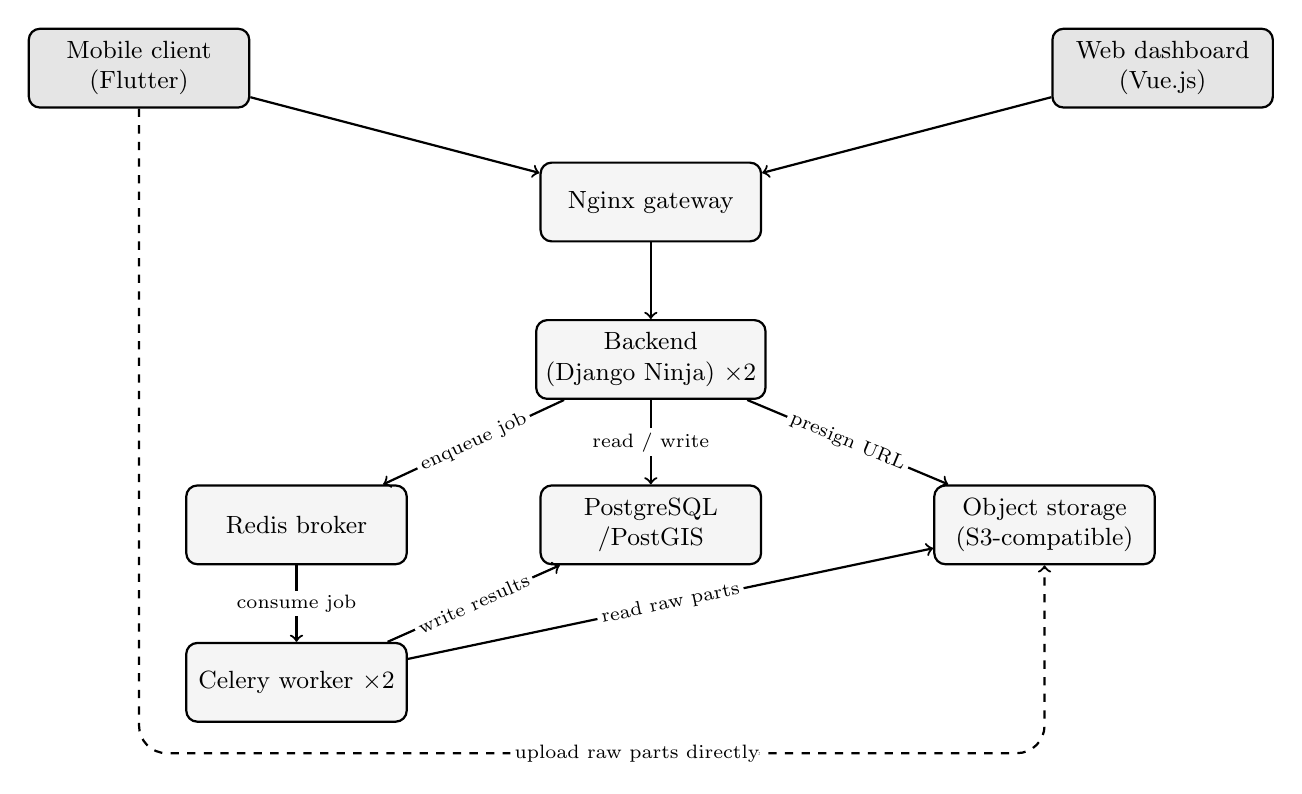
\begin{tikzpicture}[
  box/.style={draw, rounded corners, minimum width=2.8cm, minimum height=1cm, align=center, font=\small, fill=gray!8},
  ext/.style={draw, rounded corners, minimum width=2.8cm, minimum height=1cm, align=center, font=\small, fill=gray!20},
  lbl/.style={font=\scriptsize, fill=white, inner sep=1.5pt},
  ->, thick
]
\node[ext] (mobile) at (0,8)     {Mobile client\\(Flutter)};
\node[ext] (webui)  at (13,8)    {Web dashboard\\(Vue.js)};
\node[box] (gw)     at (6.5,6.3)  {Nginx gateway};
\node[box] (web)    at (6.5,4.3)  {Backend\\(Django Ninja) $\times$2};
\node[box] (redis)  at (2,2.2)    {Redis broker};
\node[box] (db)     at (6.5,2.2)  {PostgreSQL\\/PostGIS};
\node[box] (s3)     at (11.5,2.2) {Object storage\\(S3-compatible)};
\node[box] (worker) at (2,0.2)    {Celery worker $\times$2};

\draw (mobile) -- (gw);
\draw (webui)  -- (gw);
\draw (gw) -- (web);
\draw (web) -- node[lbl, sloped]{enqueue job} (redis);
\draw (web) -- node[lbl]{read / write} (db);
\draw (web) -- node[lbl, sloped]{presign URL} (s3);
\draw (redis) -- node[lbl]{consume job} (worker);
\draw (worker) -- node[lbl, sloped]{write results} (db);
\draw (worker) -- node[lbl, sloped]{read raw parts} (s3);
\draw[dashed, rounded corners=10pt]
  (mobile.south) -- (0,-0.7) -- node[lbl, pos=0.55]{upload raw parts directly} (11.5,-0.7) -- (s3.south);
\end{tikzpicture}
\caption{System Design of Mobility Diary}
\label{fig:deployment}
\end{figure*}

\subsection{The Role of Components in the trip lifecycle}
Each component owns a distinct part of the trip lifecycle. The mobile client detects movement and stores route data locally before sending it to the back end through the gateway, the system's sole external access point, which manages traffic and balances request load between the replicated backend instances. The backend, accessible through dedicated routers for authentication, data acquisition, mobility management, and privacy, validates requests, executes operations, and delegates the most resource-intensive tasks to Celery workers via a Redis broker; those workers perform human-activity-recognition inference and significant-place extraction. PostgreSQL/PostGIS stores relational and geospatial data and answers spatial queries, while the object store holds the raw sensor data uploaded by the mobile client.

Trip data passes through these components in the fixed sequence shown by the arrows in Fig.~\ref{fig:deployment}: the mobile client records the data locally; at the end of the trip it sends the essential trip data to the backend acquisition endpoint, which creates a trip record in PostgreSQL/PostGIS; the raw sensor data is then uploaded directly to the object store via pre-signed URLs; once confirmed, a Celery worker retrieves the task from the Redis queue, performs HAR inference and place mining, and writes the results back to PostGIS; finally, the mobile app and the web dashboard read the enriched diary through the same backend API.



\subsection{Functional Requirements}
Mobility Diary follows the \textit{Privacy-Aware Mobility Diary with HAR} specification. Table~\ref{tab:specmap} reproduces the requirements of that specification, both from the mandatory base application and from its optional extensions, and states for each one what the system must provide, described in terms of behaviour rather than implementation. Every requirement listed is realized by the implemented system; all but Docker Compose have a dedicated subsection later in this section and in Section III, while Docker-based deployment is reported in Section IV.

\begin{table*}[htbp]
\caption{Functional Requirements of the \textit{Privacy-Aware Mobility Diary with HAR} Specification}
\begin{center}
\begin{tabularx}{\textwidth}{p{0.24\textwidth} X}
\toprule
\textbf{Requirement} & \textbf{What the system must provide}\\
\midrule
GPS trace collection & Collect, upload, or simulate GPS traces containing at least timestamps and coordinates.\\
Daily map visualization & Display the daily mobility on a map, visually distinguishing movement segments from stops.\\
Trace segmentation & Automatically split each trace into movement and stop segments, following documented rules.\\
Mobility diary & Build a diary of significant places and time intervals that is more informative than a raw list of GPS points.\\
Basic HAR & Recognize the mobility mode, through a system activity-recognition API or a simple classifier.\\
Web dashboard & Show traces, significant places, and statistics on a web dashboard.\\
Advanced HAR & Recognize at least three mobility classes (e.g.\ walking, biking, driving, idle) from sensor and/or GPS data over a described dataset; justify the features when a machine-learning model is used; handle ambiguous cases; and evaluate the classifier with accuracy, precision, recall, and a confusion matrix.\\
Route assistant & Let the user select an origin and a destination, suggest a route based on the recognized or selected mobility mode, and update the route dynamically when the mode changes.\\
Advanced significant places & Cluster GPS points into recurring places, classify them into categories (home, university, work, gym, other, possibly with manual labels), and link them to diary segments.\\
Location privacy & Apply at least one location-privacy technique, produce a detailed private view and a shareable privacy-aware view, and measure Privacy Perturbation and Quality of Service, visualizing the trade-off.\\
Personal analytics & Provide daily and weekly charts of time spent per activity, a heatmap of the most visited places, and statistics on frequent routes, distances, and prevalent mobility modes.\\
Docker Compose & Containerize back-end, database, and front-end, and start the whole platform with a single Docker Compose command.\\
\bottomrule
\end{tabularx}
\label{tab:specmap}
\end{center}
\end{table*}

\subsection{Mobile Acquisition \& FSM}

This subsection realizes the \textit{GPS trace collection} row of Table~\ref{tab:specmap}. The mobile client tracks trips through a finite-state machine with three states: stationary, potential-motion, and active-tracking. Transitions are driven by two signals evaluated jointly: a GPS speed reading and an accelerometer-derived motion sigma value. Movement is confirmed only once both signals agree for at least 15 seconds, with GPS speed at least 0.8 m/s and sigma at least 1.2; a return to stationary instead requires a longer 120-second window, with GPS speed below 0.4 m/s and sigma below 0.8. This asymmetry is deliberate: stopping a trip should require more confidence than starting one, to avoid oscillating on noisy signals.

Sensing intensity follows the FSM state through a sampling profile. While stationary, the client samples at a low frequency and skips HAR window persistence entirely; once tracking is confirmed, GPS points, state transitions, and HAR sensor windows are all persisted locally through Drift/SQLite before any network exchange. This local-first design means a trip survives a temporary loss of connectivity, and synchronization can be retried independently of the recording itself. When the user stops a trip, the local session closes and a background synchronization queue takes over: it builds the core payload, submits it, uploads raw sensor parts with bounded parallelism, and polls the backend while enrichment runs, so the mobile UI never blocks on any of this.

\subsection{Trip Upload Pipeline}

This subsection describes the upload pipeline that carries the data behind \textit{GPS trace collection} and \textit{Basic/Advanced HAR} to the backend; the two-phase design is an engineering extension beyond the base requirements. Upload happens in two independent phases. Core ingestion carries the minimum evidence needed to reconstruct a visible trip, GPS points and state transitions, as one deterministic JSON payload verified against a stable hash, so retries are idempotent and never create duplicate trips. As soon as core ingestion succeeds, the trip is materialized in PostgreSQL/PostGIS and becomes visible to the user, regardless of whether raw sensor data has finished uploading.

Once core ingestion succeeds, the backend hands the mobile client a presigned URL for each raw sensor part, and the client uploads the compressed binary bytes directly to object storage, bypassing the backend entirely; this presign-confirm-complete protocol starts only after the core phase is confirmed, never in parallel with it. The indirection exists because inertial data is heavy: at 100 Hz, a single window is already a 500-by-6 matrix of raw samples, too large and too numerous to fit inside the core JSON payload or a synchronous API request. On the backend side, each uploaded part is confirmed individually by checking object existence, size, and a SHA-256 checksum; once every expected part has been confirmed this way, the mobile client calls a completion endpoint, and the backend marks the raw phase as queued and creates a Celery job for the final HAR processing. Splitting the upload into independent parts also lets the client retry a single failed part instead of resending an entire trip, and keeps large byte transfers off the Django web process.

Both phases are tracked by an explicit state machine stored in the database, with core and raw progressing independently through pending, receiving, received, queued, processing, completed, retryable-failure, and final-failure. The mobile app relies on this distinction directly: \texttt{core\_status=COMPLETED} means the trip is visible, while \texttt{raw\_status=COMPLETED} means the diary has been fully enriched, so the trip list never waits for model inference to finish.

\subsection{Backend Service Layer}

The backend is implemented with Django and Django Ninja. Django provides the relational model, migrations, authentication integration, and administrative interface, while Django Ninja exposes typed HTTP APIs. The backend codebase uses a service-layer architecture in which API routers remain thin and delegate domain operations to services and selectors, keeping business logic out of controllers and ORM models and making the ingestion, trip, privacy, analytics, and place-mining workflows easier to test in isolation.

The main domain objects include users, trips, GPS points, state transitions, trip ingestions, ingestion parts, HAR jobs, mobility segments, virtual stop intervals, candidate visits, and habitual places. A \texttt{Trip} corresponds to the mobility trace; \texttt{GpsPoint} stores timestamped spatial samples; \texttt{MobilitySegment} represents the diary intervals; \texttt{ActivityLabel} represents the recognized mobility mode; and \texttt{HabitualPlace} represents the significant-place abstraction. PostGIS is used for geospatial fields such as GPS points, trip paths, mobility-segment paths, visit centers, and significant-place centers; Redis is used as the Celery broker.

The API surface follows the same model. Core mobile APIs let the client create or synchronize trips, upload GPS points, upload state transitions, submit sensor windows, close trips, fetch tracks and diary segments, retrieve significant places, and request privacy-aware exports. Web APIs expose staff-oriented dashboards, user trip lists, private and privacy-aware tracks, and privacy metrics, so the same backend supports both the mobile owner-facing scenario and the web inspection scenario.

\subsection{HAR Pipeline}

This subsection realizes the \textit{Advanced HAR} and \textit{Trace segmentation} rows of Table~\ref{tab:specmap}. Once every raw sensor part for a specific trip has been uploaded and confirmed, the backend queues a Celery task for that trip, and the HAR pipeline starts automatically, without the user or the mobile app doing anything further. From there, the task works through the trip end to end: it loads the confirmed raw parts for that trip from object storage, decodes the \texttt{MDHARW1} binary windows, persists the decoded samples to a TimescaleDB hypertable so they remain queryable independently of inference, normalizes the accelerometer and gyroscope channels, runs the two-stage neural pipeline described below, corrects idle predictions using GPS speed, and finally writes the resulting mobility segments back to PostGIS, completing that trip's diary.

The neural pipeline has two stages. A 1D convolutional network first acts as a per-window feature extractor, receiving one inertial window (500 samples, 6 channels: accelerometer x/y/z and gyroscope x/y/z) at a time. The resulting embeddings are then fed to a GRU model over sequences of 32 consecutive windows, so the classifier can exploit temporal context; a single window rarely disambiguates walking from running, but a sequence usually does. The five output classes are \texttt{IDLE}, \texttt{WALKING}, \texttt{RUNNING}, \texttt{BIKING}, and \texttt{MOVING\_VEHICLE}.

Running HAR after the trip is complete, rather than window-by-window during live acquisition, is a deliberate choice: the GRU model benefits from seeing the whole trip instead of making isolated per-window decisions, and it keeps the live acquisition FSM independent from possible misclassifications. A remaining ambiguity is handled explicitly: an \texttt{IDLE} prediction never closes a trip by itself, because it may just as well be a traffic light or a train stop, and a GPS-speed correction is applied after classification to fix idle intervals where the spatial evidence clearly indicates movement.

\subsection{Significant-Place Clustering}

This subsection realizes the \textit{Advanced significant places} row of Table~\ref{tab:specmap}: how recurring GPS evidence becomes a habitual place such as home, work, or gym. The process runs in two asynchronous stages, both scoped to a single user. At the heart of the pipeline is DBSCAN, a spatial clustering algorithm; but DBSCAN alone is not enough here, because it groups points based solely on spatial proximity and has no notion of time, so it cannot distinguish a genuine stay from GPS points that simply happen to pass close to each other, such as along a road. This is why a preprocessing stage runs first, to turn raw GPS points into discrete visits before any clustering takes place.

This first stage implements a simple stay-point detection algorithm: it scans a user's GPS points in temporal order and accumulates them into a candidate visit, comparing each new point against the candidate's current centroid, the average of all coordinates accumulated so far, and discarding the point if it lies more than 75 meters from that centroid; the centroid itself is recalculated after every accepted point. Points with a reported accuracy worse than 100 meters are discarded before they can even be considered. A candidate visit becomes a confirmed visit only once it contains at least three valid points and lasts at least five minutes, measured as the difference between the timestamps of its last and first accumulated points; otherwise it is discarded without becoming a visit.

Once visits have been extracted this way, the second stage applies DBSCAN to group visits that are spatially close to each other, as distinct from isolated ones. For each visit, the algorithm checks how many other visits by the same user fall within a 100-meter radius: if at least two more are found, all of them are grouped into the same cluster, since their repeated proximity indicates that the user has returned to the same area multiple times. A visit without enough nearby visits is not assigned to any cluster and is discarded, since a single occurrence is not by itself evidence of a regularly visited place.

Before creating a new place from a cluster, mining checks whether a manually reviewed place already exists within the same 100-meter radius; if so, the cluster is reattached to that place instead, leaving its identity and label untouched. Otherwise, a new \texttt{HabitualPlace} is created, but only if the cluster spans at least two distinct calendar days; below that threshold, the cluster is discarded. A cluster observed on three or more distinct days is automatically confirmed, while one observed on only two remains a candidate place.

\subsection{Privacy-Aware Export}

This subsection realizes the \textit{Location privacy} row of Table~\ref{tab:specmap}. Privacy is implemented as a single projection pipeline rather than as separate diary-generation code paths. The detailed private diary is built once from canonical domain entities, mobility segments, virtual stop intervals, GPS points, confirmed habitual places, and HAR labels, and every privacy level is a transformation applied to that same representation.

Three levels are supported. The precise level returns the diary unchanged, for the owner's own inspection. The approximate level keeps the narrative sequence of stops and movements but rounds timestamps to five-minute boundaries, spatially approximates the movement path, replaces real place names with category-level labels, and recomputes distance on the approximated path instead of the real one. The aggregated level drops the event-level sequence entirely and instead groups activity into broad time bands (night, morning, afternoon, evening), publishing only activity patterns, distance buckets, and total durations; no coordinates and no place identities survive at this level. Because the mobile export endpoint and the web dashboard both call the same builder, a change to the privacy policy is implemented and tested in exactly one place instead of being duplicated across clients.

\subsection{Personal Analytics}

This subsection realizes the \textit{Personal analytics} row of Table~\ref{tab:specmap}. Analytics are computed from the same persisted mobility segments and habitual places used elsewhere in the diary, not from a separate aggregation pipeline. Activity duration and distance are grouped into daily and weekly buckets, mapped onto user-facing mobility categories (stopped, walking, running, cycling, vehicle), and used to derive the prevalent non-idle mode for a period. Habitual places contribute two further views: heatmap points weighted by visit count, and frequent routes computed between pairs of known places. Because these are derived views over already-enriched data, no additional background job is needed beyond the HAR and place-mining pipelines already described.

\subsection{Web Dashboard}

This subsection realizes the \textit{Web dashboard} row of Table~\ref{tab:specmap}. In addition to the mobile client, the project ships a Vite-based web dashboard aimed at authenticated users and trusted operators: trip and privacy dashboards, maps, timelines, analytics views, and inspection of privacy-aware diary projections. The web client consumes the same backend API as the mobile app wherever the two overlap, so trip, HAR, place, and privacy logic is never reimplemented for the web; it only adds staff-oriented global views that are not meaningful on a single owner's phone, such as inspecting another user's trips for demonstration and support.

\subsection{Route Assistant}

This subsection realizes the \textit{Route assistant} row of Table~\ref{tab:specmap}. The assistant lets the user pick a destination and get a route in a chosen mode (walking, cycling, driving), using the active trip's location as the route origin when a recording is in progress, or the current GPS fix otherwise.

In live mode, the route mode is not chosen manually but inferred from context: the mobile client periodically sends a current sensor window to the same backend HAR classifier used for trip enrichment, and the returned activity is mapped onto a navigation profile; walking and running both become a pedestrian route, biking becomes a cycling route, and moving vehicle becomes a driving route. This reuses the HAR vocabulary built for the diary instead of introducing a second, separate classifier, and lets route suggestions adapt automatically as the user's actual movement changes.

\section{Project's Implementation}

\subsection{Mobile Implementation}

The mobile application is implemented in Flutter. The project uses a modular structure that separates domain entities, repositories, network services, state-management Cubits, mappers, and UI pages. Acquisition-related domain models include route points, tracking events, sampling profiles, motion metrics, sensor windows, synchronization snapshots, and finite-state-machine state. This separation keeps UI concerns independent from synchronization and sensing logic.

During a trip, evidence is persisted locally before it is sent to the backend. This is essential because mobile connectivity is not guaranteed. GPS points and state transitions form the core trip evidence. HAR windows form raw evidence for final enrichment. The local database stores the matrix of each standard sensor window as a binary blob, avoiding the overhead of JSON serialization for high-frequency sensor matrices. A standard production window contains 500 samples, 6 channels, and 4 bytes per float, resulting in 12,000 bytes before compression.

When the user stops a trip, the mobile application closes the local recording session and creates or updates a persistent synchronization job. The UI can return to an idle state immediately. The synchronization queue then builds a deterministic core JSON payload, submits it to the backend, receives the corresponding ingestion and trip identifiers, uploads raw binary parts with bounded parallelism, and polls the backend while the server-side enrichment is queued or running.

\subsection{Adaptive Sampling and FSM Implementation}

This subsection provides implementation-level detail behind the finite-state machine described in Section II-C. The FSM operates on synthesized events rather than raw sensor streams, namely motion-window evaluations, GPS fixes, and timeout events, which keeps it independent from the concrete sensor runtime and easy to test in isolation. Each decision returns the next tracking state, the sampling profile to apply, and an optional transition record; every transition stores its source state, target state, timestamp, and reason.

The synchronization queue processes only authenticated jobs, uploads the core payload before any raw part, retries with backoff on failure, and relies on backend idempotency to avoid creating duplicate remote trips on retry. Raw upload concurrency is bounded to avoid saturating the device's network connection.

\subsection{Raw Sensor Binary Format}

This subsection provides implementation-level detail behind the upload pipeline described in Section II-D. The raw sensor format is a compressed binary file named according to the pattern \texttt{sensor\_windows\_part\_XXXX.bin.gz}. After decompression, the payload is little-endian and starts with the magic value \texttt{MDHARW1}. The global header contains the number of windows; each window stores start and end timestamps in UTC microseconds, sampling frequency, sample count, channel count, and the contiguous float32 sample matrix.

This format replaced a previous JSON-based representation. The binary representation reduces payload size, avoids expensive JSON parsing for dense matrices, and maps naturally to NumPy arrays in the backend. Compatibility with legacy JSON payloads is preserved where needed, but the production path uses binary float32 windows with 6 channels.

\subsection{Backend Ingestion API}

This subsection provides implementation-level detail behind the upload pipeline described in Section II-D. The ingestion API is implemented in the Django Ninja application. The core path uses \texttt{POST /api/ingestion/trips/core}. This endpoint validates the canonical hash of the payload, creates or retrieves the corresponding \texttt{TripIngestion}, materializes the \texttt{Trip}, \texttt{GpsPoint}, \texttt{StateTransition}, and route geometry records, and marks the core phase as completed.

Raw sensor ingestion follows a presign-confirm-complete protocol. The mobile client asks the backend for a presigned URL for a raw part, uploads the compressed binary object directly to the storage service, and then confirms the part. Confirmation checks object existence, size, and SHA-256 metadata. When all expected parts have been confirmed, the client calls the raw completion endpoint, and the backend marks the raw phase as queued and creates a final HAR job for Celery.

Table~\ref{tab:api} summarizes the most relevant API families. The same backend exposes additional endpoints for authentication, privacy settings, web-dashboard users, and staff-oriented inspection.

\begin{table}[htbp]
\caption{Representative API Families}
\begin{center}
\begin{tabular}{p{0.33\linewidth} p{0.52\linewidth}}
\toprule
\textbf{API family} & \textbf{Purpose}\\
\midrule
Core ingestion & Submit deterministic core evidence and create a visible trip.\\
Part presign & Obtain signed upload URLs for part-based transfer.\\
Part confirm & Confirm object-storage part availability and integrity.\\
Trip diary & Retrieve the owner-facing diary timeline.\\
Privacy export & Retrieve a privacy-aware textual/mobile export.\\
Place review & Review, confirm, reject, reactivate, or label significant places.\\
Analytics & Retrieve personal mobility analytics.\\
Route assistant & Classify a sensor window into a route mode.\\
\bottomrule
\end{tabular}
\label{tab:api}
\end{center}
\end{table}

The raw object key is deterministic. A representative simplified function is shown in Listing~\ref{lst:objectkey}. The function intentionally contains no inline explanatory comments, in accordance with the code-comment policy.

\begin{lstlisting}[language=Python,caption={Deterministic object key construction for ingestion parts.},label={lst:objectkey}]
def _object_key(base_path: str, kind: str, sequence: int) -> str:
    if kind == PartKind.SENSOR_WINDOWS:
        return f"{base_path}sensor_windows_part_{sequence:04d}.bin.gz"
    return f"{base_path}{kind}.json.gz"
\end{lstlisting}

\subsection{HAR Processing Task}

This subsection provides implementation-level detail behind the HAR pipeline described in Section II-F. HAR runs as a Celery task that claims the raw ingestion idempotently, loads and decompresses the confirmed raw parts, decodes and sorts the binary windows, and only then runs the CNN+GRU model pipeline, before writing mobility segments and marking the trip as processed.

The production path uses 6 sensor channels (accelerometer and gyroscope x/y/z); earlier design notes considered a 9-channel variant that included magnetometer samples, but the final implementation dropped the magnetometer from the HAR path while keeping compatibility code for older payloads. The worker also records detailed per-stage timing, raw storage read, gzip decompression, binary decode, normalization, classification, GPS correction, and segment database write, useful for diagnosing bottlenecks and for showing that HAR is not a monolithic synchronous endpoint. The full flow is summarized in Listing~\ref{lst:harflow}.

Immediately after decoding, and before normalization, the worker also persists the decoded samples to a TimescaleDB hypertable, one row per sample instant keyed by \texttt{(trip\_id, timestamp)}, in batches via Django's \texttt{bulk\_create}. This follows a feature-store dual-write pattern: the decoded array is used immediately for inference (the physical, un-normalized values, not the network's normalized input), and the same values are also persisted for later querying, independently of the inference outcome. The write is idempotent under task retries (\texttt{ignore\_conflicts=True} against the composite primary key), and the object-storage blobs remain the replayable source of truth; the hypertable is an additive, queryable projection, not a replacement. A separate reader, not used by this task, reconstructs windows from the hypertable for consumers that do not already hold the data in memory, such as the HAR evaluation protocol described next.

\begin{lstlisting}[language={},caption={Final HAR processing flow.},label={lst:harflow}]
load confirmed raw parts
decode MDHARW1 binary windows
persist decoded samples to TimescaleDB
normalize accelerometer and gyroscope channels
run CNN feature extraction and GRU classification
correct idle intervals using GPS speed
write mobility segments and virtual stops
mark trip as processed
queue significant-place mining
\end{lstlisting}

\subsection{HAR Evaluation Protocol}

This subsection completes the \textit{Advanced HAR} row of Table~\ref{tab:specmap} with the evaluation protocol expected for the classifier described in Section II-F. The project includes the trained Keras models and the backend/mobile integration needed to run inference over real or replayed sensor windows. For a complete experimental evaluation, the HAR model should be assessed on a labelled hold-out set using the following metrics: accuracy, precision, recall, F1-score, and confusion matrix. The expected evaluation protocol is the following: split labelled windows by recording session to avoid leakage across adjacent windows, run the CNN extractor and GRU classifier on the test sequences, compare predicted classes against ground truth labels, and report per-class metrics for the five activities.

The implemented codebase already validates the integration boundaries around HAR, including invalid-window rejection, mapping from HAR labels to navigation modes, raw binary decoding, final pipeline orchestration, and diary segment generation. These tests do not replace a dataset-level accuracy benchmark, but they verify that the application pipeline can consume HAR predictions correctly. The final report should be updated with numerical HAR metrics when the labelled evaluation run is executed.

\subsection{Significant-Place Implementation}

This subsection provides implementation-level detail behind the clustering process described in Section II-G. Visit detection scans ordered GPS points and maintains a candidate permanence cluster in memory; a cluster is flushed as a visit only once the thresholds described in Section II-G are met. The clustering step uses PostGIS's native DBSCAN over projected visit centroids when PostgreSQL/PostGIS is available, with a Python fallback for non-PostgreSQL test environments.

Each mining run deletes and regenerates non-manual candidate evidence for the user before reclustering, so stale visits never accumulate; manually reviewed places are explicitly excluded from this regeneration, and manual labels always take precedence over automatically inferred ones.

\subsection{Privacy-Aware Export Implementation}

This subsection provides implementation-level detail behind the export pipeline described in Section II-H. Privacy-aware export is implemented as a single builder function that receives a trip and a target privacy level, projects the detailed diary once, and then applies the corresponding transformation branch; both the mobile export endpoint and the web dashboard call this same builder, so the transformation rules exist in exactly one place in the codebase.

\subsection{Privacy Metrics Implementation}

This subsection provides implementation-level detail supporting Section II-H by quantifying the trade-off between privacy and quality of service. The privacy-aware dashboard computes two families of metrics. The first is Privacy Perturbation, defined as the distance between each original trajectory point and its published cell center; the system reports the mean perturbation, maximum perturbation, and number of evaluated samples. The second is Quality of Service, defined as the relative error between the private route distance and the privacy-aware route distance:

\begin{equation}
QoS_{loss} = \frac{|d_{private} - d_{published}|}{d_{private}}.
\end{equation}

For the approximate level, the spatial approximation grid uses 150-meter cells. For the aggregated level, the grid uses 400-meter cells and the diary removes event-level paths and precise places. The web dashboard exposes these metrics as comparison cards and allows previewing a different privacy level without changing the user's saved default preference.

\subsection{Personal Analytics Implementation}

This subsection provides implementation-level detail behind the analytics described in Section II-I. On the mobile side, the aggregates are exposed through a dedicated analytics page; on the web side, the same selectors back dashboard views for trips, timelines, maps, private tracks, privacy-aware tracks, and metric comparisons.

\subsection{Web Dashboard and Authentication}

This subsection provides implementation-level detail behind the web dashboard described in Section II-J. Authentication for the web client is implemented through dedicated backend account APIs, token handling, and session persistence, separate from the mobile authentication flow. The web layer consumes the same backend APIs used by the mobile client where appropriate, while adding staff-oriented global views for demonstration and analysis.

\subsection{Route Assistant Implementation}

This subsection provides implementation-level detail behind the route assistant described in Section II-K, the last item in the mapping. On the mobile side, the assistant is implemented as a dedicated Cubit, kept independent from the acquisition Cubit because route assistance is an interactive feature while acquisition is a recording lifecycle. In live mode, the backend validates the incoming window shape before calling the same HAR adapter used for trip enrichment.

\subsection{AI Usage Disclosure}

Unlike the previous subsections, this disclosure does not correspond to a row of Table~\ref{tab:specmap}; it is an administrative disclosure required independently of the functional specification. The project rules explicitly require transparency regarding AI-tool usage and restrict comments in source code to the beginning of files and to the beginning of functions or methods. The implemented codebase follows this convention in the reviewed modules: explanatory comments are placed in module headers or function-level docstrings, while significant inline commentary is avoided.

During the preparation of this technical report, AI-based assistance was used only as a documentation-support tool. In particular, OpenAI Codex was used to help organize the report structure, reformulate technical explanations in academic English, and align the written description with the implemented architecture. The submitted source code was not generated to a significant extent by AI tools, and all implementation choices, APIs, data models, and programming constructs were reviewed and understood by the author. This disclosure is included in accordance with the project AI policy.

\section{Results}

\subsection{Functional Results}

The implemented system provides a complete path from mobile sensing to diary visualization. A user can record a trip on the Flutter application, store the evidence locally, stop the trip without waiting for heavy backend processing, synchronize the core trip evidence, upload raw sensor evidence, and later inspect the enriched diary. The backend materializes route geometry, GPS evidence, state transitions, mobility segments, significant places, and privacy-aware exports. The mobile and web clients can then display trip lists, trip details, maps, timeline entries, analytics, place information, and privacy-aware diary views.

The main qualitative result is the successful separation between visibility and enrichment. A trip can become visible after core ingestion, while raw HAR processing and significant-place mining continue asynchronously. This behavior is appropriate for a context-aware mobile system because it reduces perceived latency and prevents the user interface from depending on machine-learning processing time.

Table~\ref{tab:extensions} summarizes the coverage of the optional components described in the Privacy-Aware Mobility Diary proposal. The strongest implemented extensions are advanced significant-place recognition, privacy-aware diary generation with metrics, personal analytics, route assistance, and Docker-based deployment.

\begin{table}[htbp]
\caption{Coverage of Optional Project Components}
\begin{center}
\begin{tabular}{p{0.38\linewidth} p{0.47\linewidth}}
\toprule
\textbf{Component} & \textbf{Implemented coverage}\\
\midrule
Advanced HAR & CNN+GRU inference pipeline over inertial windows; integration tests and diary use.\\
Route assistant & Destination search, route mode selection, live HAR-based mode adaptation.\\
Advanced significant places & Stay detection, PostGIS DBSCAN clustering, manual labels, diary overlay.\\
Location privacy & Precise, approximate, and aggregated views with spatial approximation and QoS metrics.\\
Personal analytics & Time by activity, heatmaps, prevalent mode, frequent routes.\\
Docker Compose & Backend, database, Redis, worker, gateway, and deployment compose files.\\
\bottomrule
\end{tabular}
\label{tab:extensions}
\end{center}
\end{table}

\subsection{Reliability Evaluation}

Reliability was evaluated through the ingestion design and through automated tests. The mobile application stores evidence locally before synchronization, so temporary connection failures do not immediately imply data loss. The backend ingestion workflow is idempotent, uses stable hashes for core payloads, and separates part upload from part confirmation. Raw evidence is divided into parts, allowing partial retries. The backend state model distinguishes pending, receiving, received, queued, processing, completed, retryable failure, and final failure states.

The architecture also handles active-trip consistency. The backend maintains the concept of a single active recording per trip owner and associates the recording with an origin device. This prevents two devices from recording conflicting active trips for the same account. Heartbeats and abandonment rules allow stale recordings to be released after a defined period or when the origin device reports that it can no longer resume the local session.

\subsection{Testing Strategy}

The repository contains backend and mobile tests covering the most important domain boundaries. Backend tests verify ingestion APIs, ingestion services, raw sensor codec behavior, trip services, trip selectors, place services, route-assistant services, reload services, analytics selectors, diary export behavior, and architecture boundaries. Account tests verify registration, web authentication, web user APIs, and privacy settings APIs. Mobile tests cover Cubits, repositories, DTOs, Drift database behavior, acquisition runtime components, synchronization queue behavior, FSM behavior, motion metrics, HAR sensor windows, UI widgets, and architecture import boundaries.

Table~\ref{tab:tests} summarizes representative tested areas.

\begin{table}[htbp]
\caption{Representative Validation Areas}
\begin{center}
\begin{tabular}{p{0.27\linewidth} p{0.58\linewidth}}
\toprule
\textbf{Area} & \textbf{Validation focus}\\
\midrule
Ingestion API & Core submission, raw part lifecycle, status transitions, idempotent behavior\\
Raw sensor codec & Binary payload parsing, legacy compatibility, invalid payload handling\\
HAR pipeline & Final processing orchestration, segment generation, timing instrumentation\\
Significant places & Visit detection, clustering, manual review preservation, user scoping\\
Privacy export & Precise, approximate, and aggregated diary transformations\\
Mobile acquisition & FSM behavior, sensor windows, local database, synchronization queue\\
Architecture boundaries & Import rules and separation between service, selector, API, and UI layers\\
\bottomrule
\end{tabular}
\label{tab:tests}
\end{center}
\end{table}

\subsection{Context-Awareness Evaluation}

The project satisfies the main properties expected from a context-aware system. It senses environmental and user-related context through GPS and inertial sensors. It interprets context through an acquisition finite-state machine, HAR classification, stop detection, and significant-place mining. It adapts behavior to context by changing sensing intensity across stationary, potential-motion, and active-tracking states. It produces user-facing context representations through trip timelines, mobility categories, place labels, and analytics. It also adapts disclosure according to privacy context by transforming the diary into precise, approximate, or aggregated forms.

The architectural distinction between operational context and semantic context proved especially important. The FSM uses simple, robust signals to decide whether tracking should be active, while HAR assigns semantic activity labels after sufficient evidence has been collected. This prevents the system from prematurely closing a trip because of an isolated idle prediction and allows richer temporal models to operate after the full trip is available.

\subsection{Performance-Oriented Design Outcomes}

Although the final evaluation was primarily functional, several implementation choices directly improve performance. The binary raw sensor format removes JSON overhead for high-frequency matrices. Gzip compression reduces network and storage volume. Direct object-storage uploads prevent the Django web process from handling large raw bytes. Celery workers isolate CPU-intensive model execution from request-response APIs. PostGIS performs spatial operations inside the database, including route geometry handling and DBSCAN-based clustering. Local SQLite persistence allows the mobile client to batch and retry synchronization rather than issuing a fragile stream of tiny network requests.

The system is therefore designed to scale beyond a single demonstration device. The intended deployment can run multiple web replicas behind a gateway, multiple Celery workers consuming the queue in parallel, PostgreSQL/PostGIS for structured geospatial persistence, Redis for task coordination, and S3-compatible storage for raw evidence. This does not remove the need for production monitoring, but it establishes a clear path from prototype to a more robust service.

\subsection{Summary}

The final system demonstrates a complete context-aware mobility pipeline. It records context on a mobile device, synchronizes it reliably, enriches it asynchronously, mines recurring places, and exposes the result through privacy-aware views. The strongest result is the integration of mobile sensing, distributed ingestion, geospatial storage, machine-learning enrichment, and privacy projection into a coherent architecture. This combination makes Mobility Diary suitable as a course project for Context-Aware Systems because it addresses sensing, interpretation, adaptation, and user-facing contextual services within a single implemented platform.

\section*{Acknowledgment}

This project was developed for the Context-Aware Systems course at the University of Bologna, held by Prof. Marco Di Felice and Prof. Angelo Trotta.

\begin{thebibliography}{00}
\bibitem{flutter} Flutter documentation, ``Build apps for any screen,'' Google. [Online]. Available: \url{https://docs.flutter.dev/}
\bibitem{django} Django Software Foundation, ``Django documentation.'' [Online]. Available: \url{https://docs.djangoproject.com/}
\bibitem{postgis} PostGIS Project Steering Committee, ``PostGIS documentation.'' [Online]. Available: \url{https://postgis.net/documentation/}
\bibitem{celery} Celery Project, ``Celery distributed task queue documentation.'' [Online]. Available: \url{https://docs.celeryq.dev/}
\bibitem{ieee} IEEE, ``IEEE conference templates.'' [Online]. Available: \url{https://www.ieee.org/conferences/publishing/templates.html}
\end{thebibliography}

\end{document}
